\documentclass[10pt,compress]{beamer}
%\documentclass[fleqn,xcolor=dvipsnames]{beamer}
\usetheme{Madrid}
%\usetheme{Boadilla}
%\usetheme{default}
%\usetheme{Warsaw}
%\usetheme{CambridgeUS}
%\usetheme{Sybila}
%\usetheme[hideothersubsections]{Berkeley}
%\usetheme[hideothersubsections]{PaloAlto}
%%\usetheme[hideothersubsections]{Goettingen}
%\usetheme{CambridgeUS}
%\usetheme{Bergen} % This template has nagivation on the left
%\usetheme{Frankfurt} % Similar to the default with an extra region at the top.

% Uncomment the following line if you want page numbers and using Warsaw theme%
%\setbeamertemplate{footline}[page number]

\definecolor{aggiemaroon}{RGB}{80,0,0} % Official RGB code for aggie maroon
\usecolortheme[named=aggiemaroon]{structure}
\useoutertheme{shadow}
\useinnertheme{rounded}
\setbeamertemplate{navigation symbols}{}
\setbeamerfont{structure}{family=\rmfamily,series=\bfseries}
\usefonttheme[stillsansseriftext]{serif}

\usepackage{amsmath}
\usepackage{caption}
\usepackage{graphicx,comment}
\usepackage[english]{babel}
\usepackage{graphicx}
\usepackage{rotating}
\usepackage{multicol}
\usepackage{hyperref}
\usepackage{enumerate}
\usepackage{tikz}
\usepackage{graphicx}
\usepackage{bm}

% \usebackgroundtemplate{
% \tikz\node[opacity=0.025, rotate = 0] {\includegraphics[height=\paperheight,width=\paperwidth]{TAM-Logo.png;}
%{\includegraphics[height=1in,width=1in]{TAM-Logo.png}};}


\title[Texas A\&M University]{Efficiency comparison of DDP and SQP on trajectory optimization}

\author [Yeh]{Ta-Wei Yeh}

\date[ 04/25/2024]{April 25, 2024}

\institute[Texas A\&M U.] % (optional, but mostly needed)
{Texas A\&M University, College Station, TX \\
 
\includegraphics[scale=0.60]{./images/TAM-Logo1.png} \\ [0.0 cm]
 }



\AtBeginSection[]
{
  \begin{frame}<beamer>
    \frametitle{Section \thesection}
    \tableofcontents[currentsection,currentsubsection]
  \end{frame}
}

\begin{document}

\begin{frame}
\titlepage
\end{frame}

% \begin{frame}{Overview}
% \tableofcontents
% \end{frame}

\section{Problem}

\subsection{Trajectory optimization}

\begin{frame}{What is trajectory optimization? }
\vspace{0.5 cm}
\begin{enumerate}
\item Trajectory optimization is an optimal control problem that outputs an optimal control trajectory considering a dynamical system over a period of time.  
\item In an optimal control problem, the decision variables need to consider the system dynamics constraint which could easily be nonlinear in the real world. 
\end{enumerate}

\begin{figure}[b]
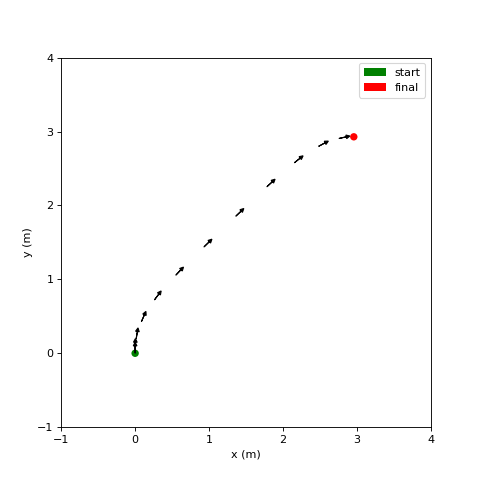
\includegraphics[width=5cm]{./images/no_obstacles.png}
\centering
\caption{Trajectory optimization without obstacles }
% \label{trajectory-no-obstacle}
\end{figure}
\end{frame}

\subsection{Problem formulation}

\begin{frame}{Problem formulation}

The trajectory optimization problem is usually formulated as, 
\begin{align}
    \min_{\textbf{x}, \textbf{u}} \quad & \int^{T}_{t=0} l(\textbf{x}_t, \textbf{u}_t) + l^f(\textbf{x}_{T}) \\
    s.t. \quad & \Dot{\textbf{x}_t} = f(\textbf{x}_t, \textbf{u}_t) \\
    & \textbf{x}_{t=0} = \textbf{x}_0 \\
    & g(\textbf{x}_t, \textbf{u}_t) \leq 0
\end{align}

\begin{itemize}
    \item $l$ is the cost-to-go function \\
    \item $l^f$ is the final cost function which considers the final state \\
    \item $\textbf{x}_t$ is the state variables (e.g. positions and orientation) at time t \\
    \item $\textbf{u}_t$ is the control input (e.g. forward speed and angular speed) at time t \\
    \item $T$ is the total control time horizon \\
    \item $f$ is the differential equation of the system dynamic model \\
    \item $\textbf{x}_0$ is the initial state \\
    \item $g$ is the inequality constraint which could include trajectory obstacles 
\end{itemize}
% where $l$ is the cost-to-go function, $l^f$ is the final cost function which considers the final state, $\textbf{x}_k$ is the state variables (e.g. positions and orientation) at time k, $\textbf{u}_k$ is the control input (e.g. forward speed and angular speed) at time k, $N$ is the control time horizon, $f$ is the system dynamic model, $\textbf{x}_0$ is the initial state, and $g$ is the inequality constraint which could include trajectory obstacles. 
\end{frame}

\begin{frame}{Trajectory with obstacles}

When function $g$ considers trajectory obstacles, it will become nonlinear. 

\begin{figure}[t]
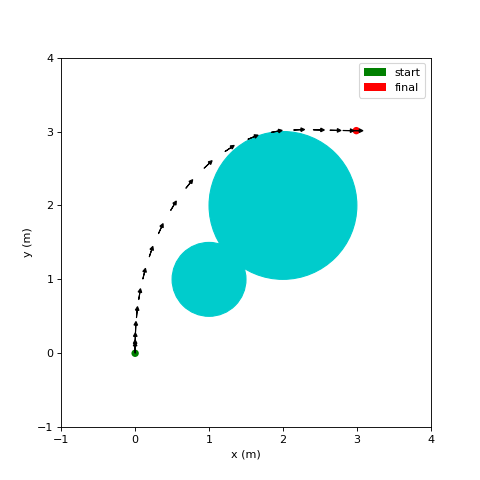
\includegraphics[width=6cm]{./images/with_obstacles.png}
\centering
\caption{Trajectory with obstacles }
\end{figure}

\end{frame}

\section{Methods}

\subsection{SQP}

\begin{frame}{Sequential Quadratic Programming}
\begin{enumerate}
\item Definition: \\
It is an iterative method to solve a constrained nonlinear problem. Each iteration solves a sub-problem which optimizes the quadratic objective function and the linearization of the constraints. 
\end{enumerate}

\begin{figure}
    \centering
    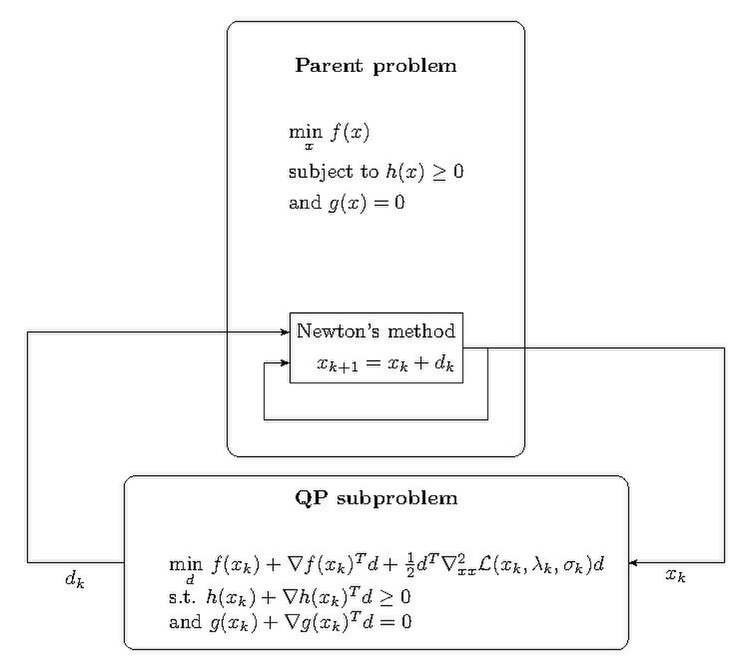
\includegraphics[height=.6\textheight]{images/SQP_schematic.pdf.jpg}
    \caption{SQP schematic}
    \label{fig:sqp-schematic}
\end{figure}

\end{frame}

\begin{frame}{How to consider dynamic function? }
    \begin{minipage}[c]{0.5\linewidth}
        \begin{enumerate}
            \item Discretizing the dynamic function
            \begin{enumerate}
                \item Single shooting
                \item Multiple Shooting
                \item Collocation
            \end{enumerate}
            \item Multiple Shooting \\
            Instead of predicting the entire trajectory (single shooting), it breaks it into many shorter segments. Each segment predicts the next state based on the current state and control. 
        \end{enumerate}
    \end{minipage}
    \begin{minipage}[c]{0.45\linewidth}
    \vspace{0.2 cm}
    \begin{figure}[h]
        % \centering
        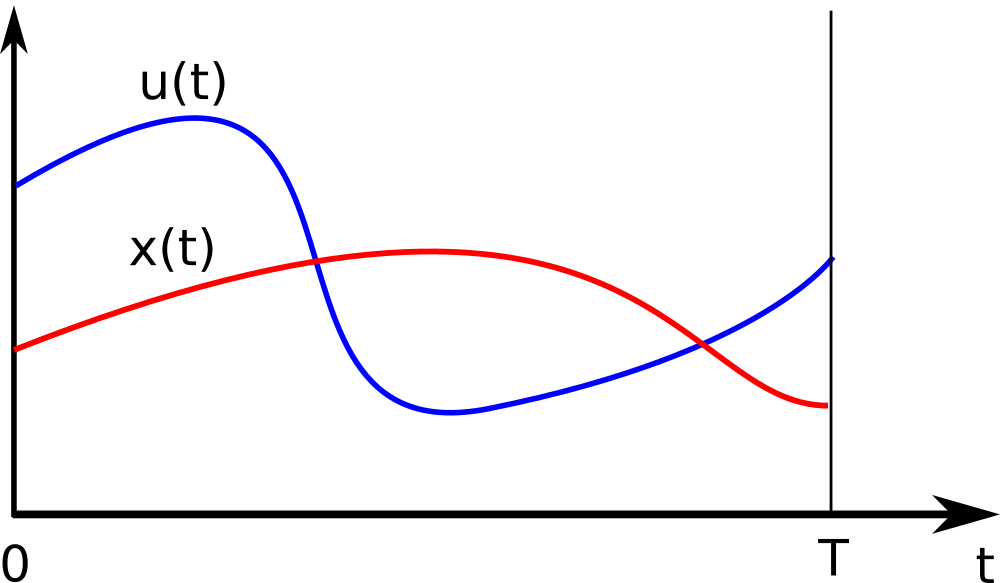
\includegraphics{images/xu_cont.png}
        \caption{Continuous state and control}
    \end{figure}
    
    \begin{figure}[h]
        % \centering
        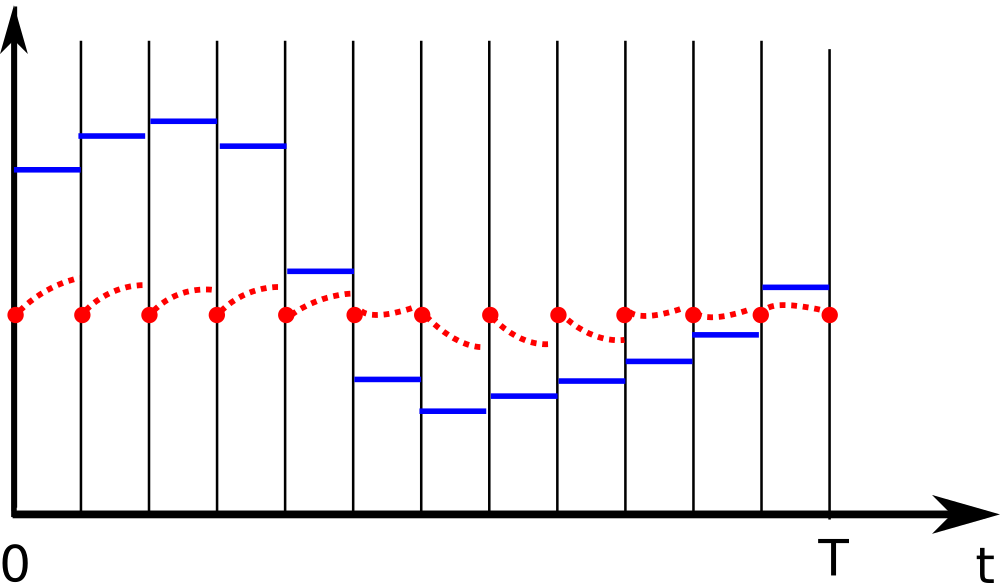
\includegraphics{images/xu_gap.png}
        \caption{Discretized state and control}
    \end{figure}
    \end{minipage}
\end{frame}

\begin{frame}{Trajectory optimization after discretization}

\begin{itemize}
    \item The objective function size expanded after discretizing the entire trajectory using multiple shooting methods. The new optimization becomes
    \begin{align}
        \min_{\textbf{u}} \quad & \sum^{N-1}_{k=0} l(\textbf{x}_k, \textbf{u}_k) + l^f(\textbf{x}_N) \\
        s.t. \quad & \textbf{x}_{k+1} = \textbf{x}_k + dt \cdot f(\textbf{x}_{k}, \textbf{u}_{k}), \quad k = [0, N-1] \\
        & \textbf{x}_{k=0} = \textbf{x}_0 \\
        & g(\textbf{x}_k, \textbf{u}_k) \leq 0, \quad\quad k=[0, N]
    \end{align}
    \item where  $dt$ is the time step, $N$ is the time horizon given by $T/dt$. 
\end{itemize}
    
\end{frame}

\subsection{DDP}

\begin{frame}{Differential Dynamic Programming}
\begin{enumerate}
\item DDP transforms the large problem into a succession of low-dimensional sub-problems. The method is based on Bellman's Principle of Optimality which the current sub-problem requires the best decision from the previous sub-problem. 
\item Thus, instead of optimizing the entire trajectory all at once, each sub-problem solves the control problem at a single time step. And the objective function becomes a value function, 
\end{enumerate}

\begin{align*}
    V_k(\textbf{x}) & = \min_{\textbf{u}} \sum^{N-1}_{j=k} l(\textbf{x}_j, \textbf{u}_j) + l^f(\textbf{x}_N) \\
    & = \min_{\textbf{u}} l(\textbf{x}_k, \textbf{u}) + V_{k+1}(f(\textbf{x}, \textbf{u})) \\
\end{align*}
\hspace{3.2 cm} where $V_N(\textbf{x}) = l^f(\textbf{x})$. 

\end{frame}

\begin{frame}{Differential Dynamic Programming Algorithm}
    \begin{enumerate}
        \item Backward Pass \\
        Solved the value function as a quadratic problem, which creates control step directions. Thus, creates a new nominal trajectory. 
        \item Forward Pass \\
        Ensures the feasibility of the new nominal trajectory and decreases cost function by using the trust-region method. 
    \end{enumerate}

    \begin{figure}
        \centering
        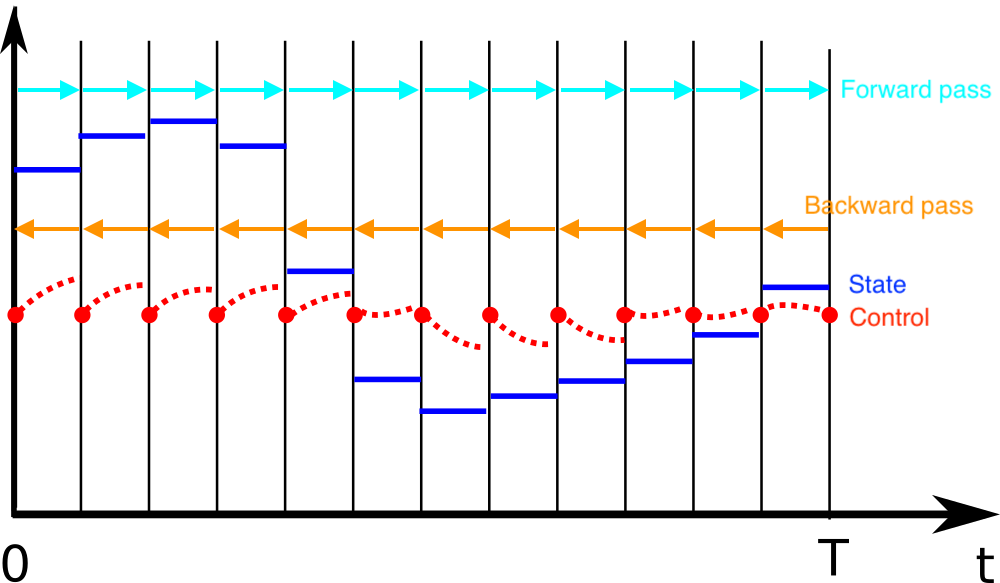
\includegraphics[width=8 cm]{images/xu_gap_ddp.png}
        \label{fig:ddp-schematics}
        \caption{DDP Schematics}
    \end{figure}
\end{frame}



\section{Result}

\begin{frame}{Convergence time comparison}

\begin{minipage}[t]{0.45\linewidth}
    \begin{itemize}
        \item {DDP Convergence time: \\ 1.27 seconds. }
    \end{itemize}
    \begin{figure}[h]
        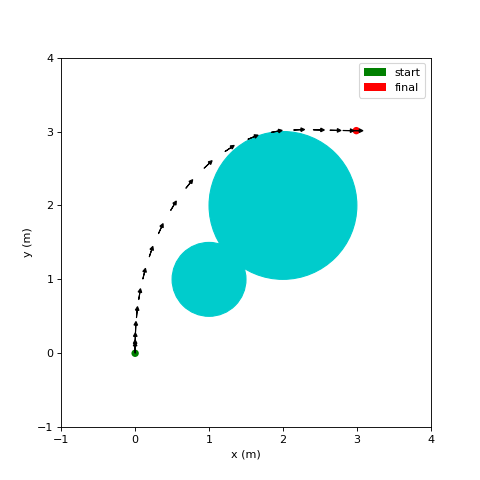
\includegraphics[width=5 cm]{./images/with_obstacles.png}
        \centering
        \caption{DDP trajectory with obstacles}
    \end{figure}
\end{minipage} \hspace{1cm}
\begin{minipage}[t]{0.45\linewidth}
    \begin{itemize}
        \item {SQP Convergence time: \\ 71.97 seconds.} 
    \end{itemize}
    % \medskip
    % \hspace{2cm}
    \begin{figure}[h]
        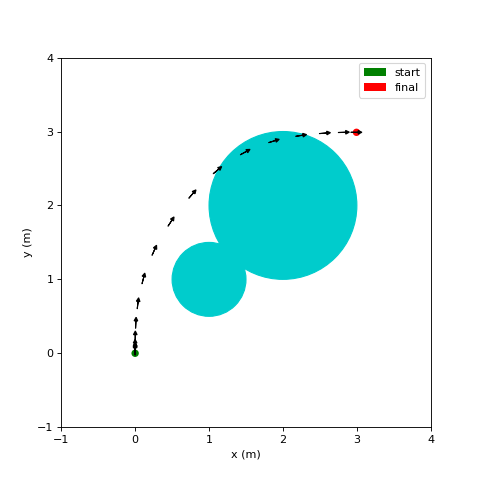
\includegraphics[width=5 cm]{./images/sqp_T5_constrained.png}
        \centering
        \caption{SQP trajectory with obstacles}
    \end{figure}
\end{minipage}

\end{frame}



\section{Conclusion}

\begin{frame}{Conclusion}
\begin{enumerate}
\item DDP decreases the trajectory optimization problem to a lower dimension problem which greatly improves the convergence speed. 
\item SQP method could be optimized with the objective Hessian and Jacobian matrix. Moreover, considering the sparsity would accelerate the convergence speed as well. For example, the professional SQP solver, SNOPT would handle this option. 
\end{enumerate}
\end{frame}


%------------------------------------------------

\begin{frame}
\frametitle{References}
% Beamer does not support BibTeX so references must be inserted manually as below

\footnotesize{
\begin{thebibliography}{99} 

\bibitem[Xie 2017]{p1} Z. Xie, C. K. Liu and K. Hauser
\newblock Differential dynamic programming with nonlinear constraints
\newblock 2017 IEEE International Conference on Robotics and Automation (ICRA)

\bibitem[Lantoine 2012]{p1} Lantoine, G., Russell, R.P
\newblock A Hybrid Differential Dynamic Programming Algorithm for Constrained Optimal Control Problems
\newblock Part 1: Theory. J Optim Theory Appl 154, 382–417 (2012). 

\bibitem[casadi-optimal-problem]{p1} CasADi - Blog - Optimal control problems in a nutshell
\newblock https://web.casadi.org/blog/ocp/
\end{thebibliography}
}
\end{frame}

%------------------------------------------------

\begin{frame}{}
  \centering \Huge
  \emph{Thank You!}
\end{frame}

%----------------------------------------------------------------------------------------


\end{document}


\end{document}
